
\chapter{Experiments} % Main chapter title

\label{ch:05} % Change X to a consecutive number; for referencing this chapter elsewhere, use \ref{ChapterX}
The experiments are performed on two normal inference tasks: normal inference based on depth image and guided normal inference based on RGB-D image. Prior works for normal estimation using very deep networks. For a single object surface normal detection as stated in this thesis, the given methods has a similar performance but only with $ 1/10 $ size.

The model is trained with PyTorch 1.10.2, CUDA 10.2.89, GPU with single NVIDIA GEFORCE GTX 1080Ti.


%% nnnn exp
\section{Surface Normal Inference based on Depth Map}
The goal of surface normal inference is to calculate the tangent surface normal map $ N $ from a single depth map $ D $. A network named Gated Convolution Neural Network (GCNN) ( \ref{gcnn}) is trained and is compared with similar approaches. We evaluate the performance of the model in dataset ``synthetic50-5" introduced in  \ref{ch:04} including 5K depth maps with size  $ 512\times512\times3 $ for training. All the depth maps add simulated noise as introduced in \ref{sec:noise}. The training pipeline use batch size $ 8 $,  Adam optimizer (\cite{adam}), learning rate of  $ 1\times10^{-3} $, penalty-l2 loss(see \ref{sec:loss}). The output is directly the tangent normal in range $ \left[-1,1\right] $. The output and input has the same shape. 

\subsection{Qualitative Evaluation}

The visual evaluation on model GCNN shown in Figure \ref{fig:gcnn-eval-synthetic-full}. 

%% a detailed analyis of this figure
It is 

The evaluation visualization on test dataset is shown in Figure \ref{fig:gcnn-eval-synthetic}. Figure \ref{fig:gcnn-eval-synthetic-zoom-in} zooms in the hindhead area of the dragon object which provides a closer comparison with the ground-truth.
\begin{figure}[th]
	\centering
	\begin{subfigure}[b]{0.15\linewidth}
		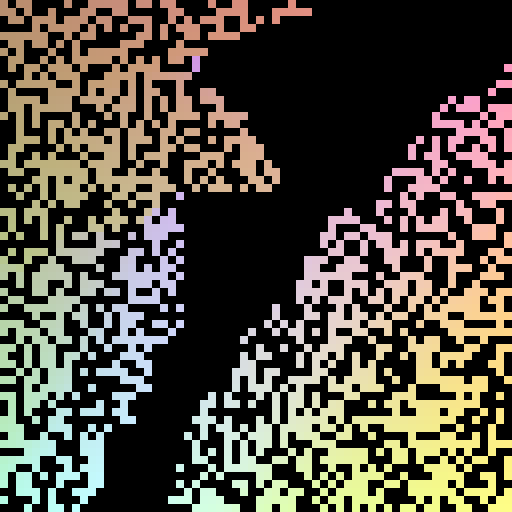
\includegraphics[width=\linewidth]{./Figures/comparison/eval_2_input.png}
		\caption{Input}
	\end{subfigure}
	\begin{subfigure}[b]{0.15\linewidth}
		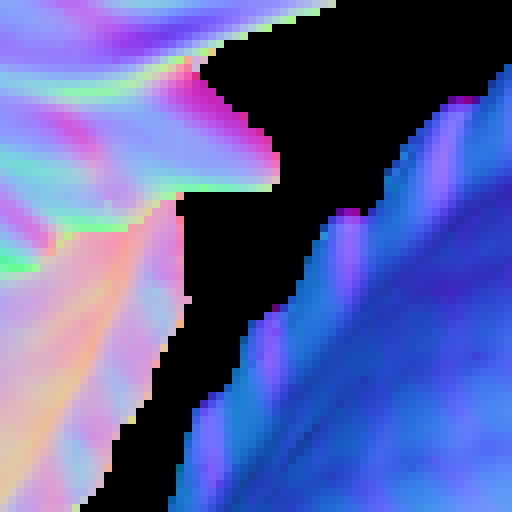
\includegraphics[width=\linewidth]{./Figures/comparison/eval_2_normal_GT.png}
		\caption{GT}
	\end{subfigure}
		\begin{subfigure}[b]{0.15\linewidth}
		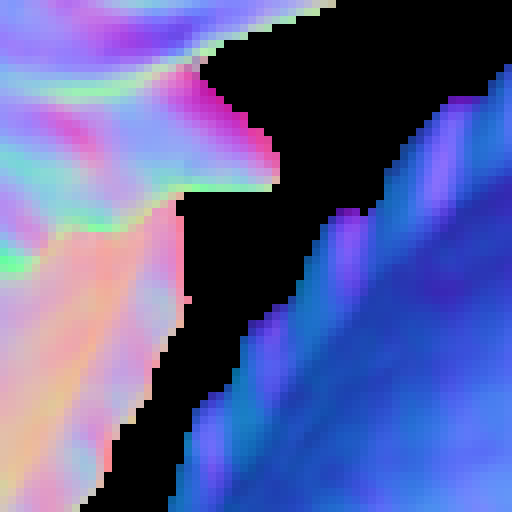
\includegraphics[width=\linewidth]{./Figures/comparison/eval_2_normal_GCNN.png}
		\caption{GCNN}
	\end{subfigure}
		\begin{subfigure}[b]{0.15\linewidth}
		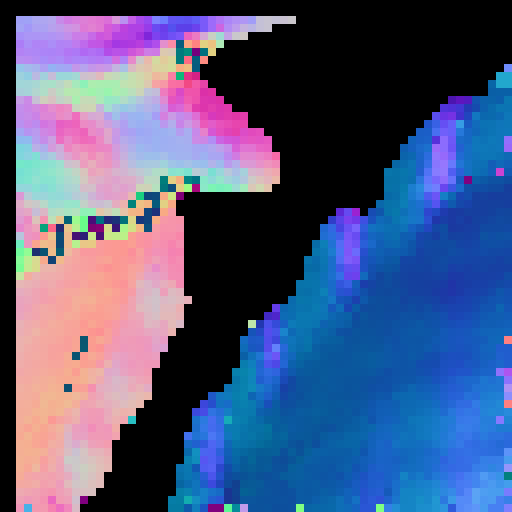
\includegraphics[width=\linewidth]{./Figures/comparison/eval_2_normal_SVD.png}
		\caption{SVD}
	\end{subfigure}
	\begin{subfigure}[b]{0.15\linewidth}
	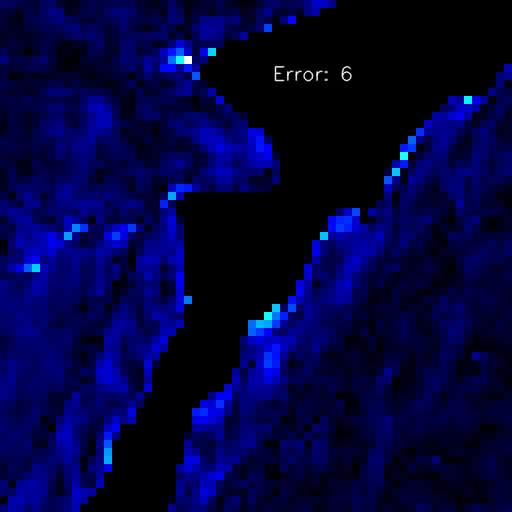
\includegraphics[width=\linewidth]{./Figures/comparison/eval_2_error_GCNN.png}
	\caption{}
	\end{subfigure}
	\begin{subfigure}[b]{0.15\linewidth}
		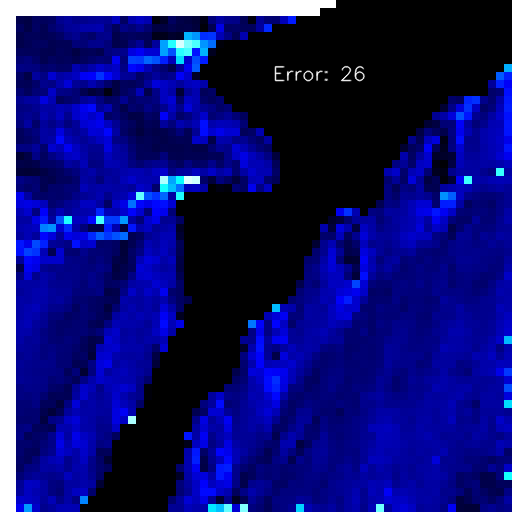
\includegraphics[width=\linewidth]{./Figures/comparison/eval_2_error_SVD.png}
		\caption{}
	\end{subfigure}
	\caption{Zoom in of dragon object evaluation.}
	\label{fig:gcnn-eval-synthetic-zoom-in}
\end{figure}



The evaluation visualization on real dataset is shown in Figure \ref{fig:gcnn-eval-real}
\begin{figure}[th]
	\centering
	\begin{subfigure}[b]{0.24\linewidth}
		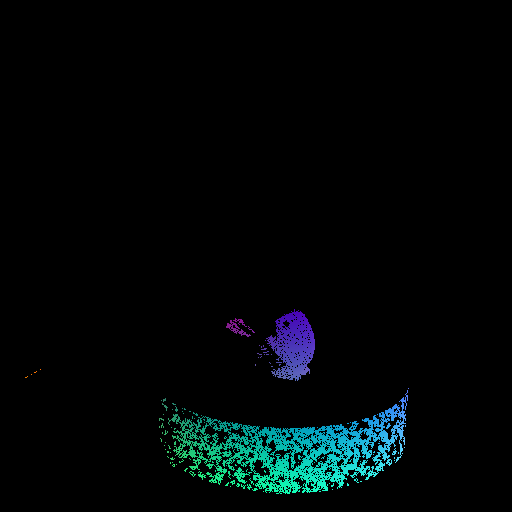
\includegraphics[width=\linewidth]{./Figures/gcnn-real/fancy_eval_1_point_cloud_noise.png}
		\caption{point cloud}
	\end{subfigure}
	\begin{subfigure}[b]{0.24\linewidth}
		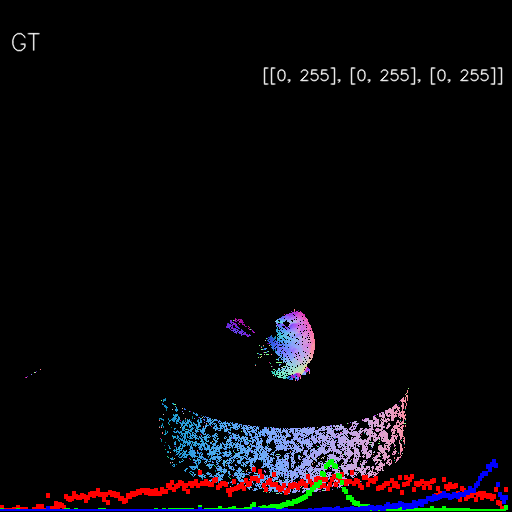
\includegraphics[width=\linewidth]{./Figures/gcnn-real/fancy_eval_1_groundtruth.png}
		\caption{ground-truth}
	\end{subfigure}
	\begin{subfigure}[b]{0.24\linewidth}
		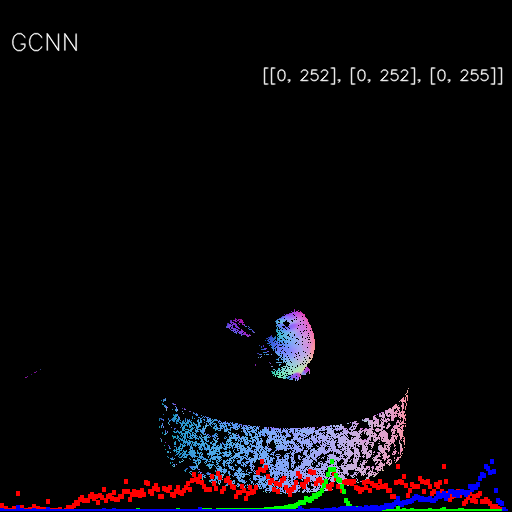
\includegraphics[width=\linewidth]{./Figures/gcnn-real/fancy_eval_1_normal_GCNN.png}
		\caption{GCNN}
	\end{subfigure}
	\begin{subfigure}[b]{0.24\linewidth}
		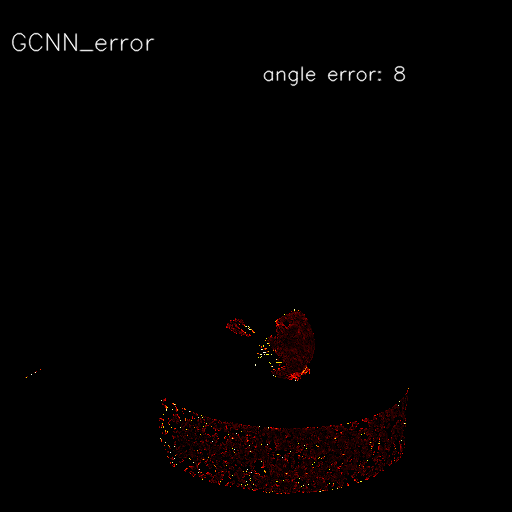
\includegraphics[width=\linewidth]{./Figures/gcnn-real/fancy_eval_1_error_GCNN.png}
		\caption{Angle Error}
	\end{subfigure}
	\caption{Evaluation on Real Dataset}
	\label{fig:gcnn-eval-real}
\end{figure}



\subsection{Quantitative Evaluation }





The evaluation result on test scenes is shown in Figure \ref{fig:scatter-gcnn}.
The GCNN based method has angle error between 5 to 15 degrees in both type of inputs. The error trends to higher with point number decrease. It is because the less points in the point cloud, the more detail is hided due to the insufficient of resolution. Therefore the recorded surface based on the point cloud is more coarse, which also increase the difficulty of the normal inference.

\begin{figure}[h!]
	\centering
	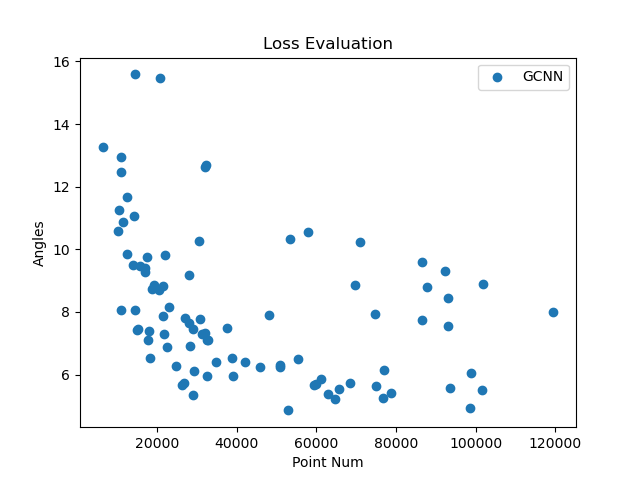
\includegraphics[width=.4\textwidth]{./Figures/scatter-gcnn-no-noise.png}
	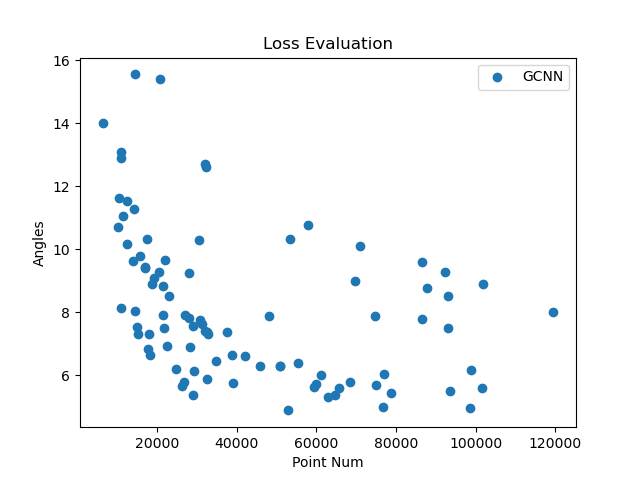
\includegraphics[width=.4\textwidth]{./Figures/scatter-gcnn-noised.png}
	\caption{Evaluation of average angular loss on the whole test dataset with 90 scenes. The x-axis indicates the point number, the y-axis indicates the angles. The \textbf{Left} one using point cloud without noise, the \textbf{right} one has noise.}
	\label{fig:scatter-gcnn}
\end{figure}




\subsection{Speed}


%% resng
\section{Guided Gated Convolution Neural Network for Normal Inference }

The inference result of guided-GCNN model is shown in Figure \ref{fig:ng-eval-synthetic}. With adding the information of a gray-scale image, the model is able to sharpen the details over the whole scene. 




\section{Guided Gated Convolution Neural Network for Normal Inference }

From the Figure \ref{fig:normal-histo-diff} we can observe the normal difference between ground-truth and GCNN predicted normals in another dimension. It separates the interval $ \left[ -1,1 \right] $, which is exactly the range of normal vector, to 256 sections. Then it counts the number of points locates in each section for 3 axes.  The 3 axes are fitted quit well in most of interval but other than $ \left[ -0.25,0.25 \right] $ for x and y axes and  interval close to $ -1 $ for z axis. Therefore a further constraint can be considered to the loss function related to the normal difference shown in this figure.

It is faulty that almost no normal has -1 z-component in GCNN predicted normal map. The reason?
\begin{figure}[h!]
	\centering
	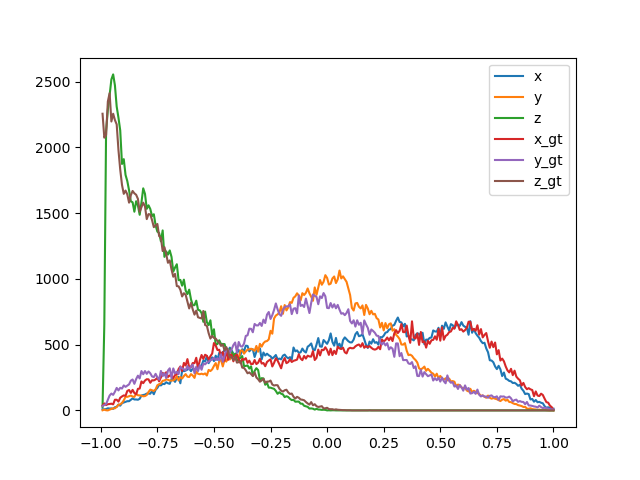
\includegraphics[width=\linewidth]{./Figures/normal-histo-diff.png}
	\caption{The normal difference of between GCNN and ground-truth in x, y, z-axis respectively. The y axis indicates the number of points, x axis indicates the value of normal in x/y/z axis. (The chart is based on the "dragon" scene showing above)}
	\label{fig:normal-histo-diff}
\end{figure}


\newpage 
\section{model comparison}
This section evaluates the proposed models with the neighbor-based model and make comparison with each other.

